\chapter{Implementation}
\label{chap:implementation}

\section{Wumpus Platform Robot}
\label{sec:wumpus_platform}
The GolfBot's development started with the Wumpus platform, a pre-existing robot that provided a solid mechanical and electrical base. This section details the initial specifications of the platform, its condition as received, and the critical modifications and improvements that were made.

\subsection{Initial Design and Specifications}
\label{ssec:initial_design}
The Wumpus robot, developed at Maynooth University, is a differential-drive robot. In its original configuration, it was controlled by a Raspberry Pi 4 running ROS 2. The power system was built around a 36V battery, which supplied two VESC motor controllers for the brushless \gls{DC} motors. The platform also included three DC-DC converters: two specifically for the VESC controllers, and a third to step the voltage down to 12V and 5V for the main controller and other peripheral electronics.

\subsection{Base Platform Condition}
\label{ssec:base_condition}
Upon initial inspection, the platform had two key issues that needed to be addressed. First, one of the VESC controllers had a recurring power-up problem. To ensure reliable operation, I installed a dedicated kill switch to control its power flow directly (shown in Figure \ref{fig:appendix_killswitch} in the Appendix). Second, the motor settings were configured for high-speed performance (minimum 900 ERPM), which made the robot uncontrollable at the low speeds required for divot inspection and repair. Using the VESC tool, an open-source configuration software, I lowered the minimum motor speed to 100 ERPM (see Figure \ref{fig:appendix_vesc_tool} in the Appendix). This adjustment was crucial for enabling the precise, low-speed maneuvers needed for the project.

\subsection{Modifications and Improvements} ter J4012, which features a powerful NVIDIA Jetson Orin 16GB module suitable for edge AI computing. I then integrated the following key hardware components:
\begin{itemize}
    \item An Intel RealSense D435i stereo camera for visual and depth data.
    \item An Ardusimple SimpleRTK2B RTK GPS module for high-accuracy localization.
    \item An Arduino Uno microcontroller to manage the dispenser motor and IMU.
    \item A BNO055 IMU sensor for orientation tracking.
    \item An A4988 stepper motor driver and a NEMA 17 stepper motor to actuate the dispenser.
    \item A custom-designed and 3D-printed auger dispenser for the sand-seed mixture.
\end{itemize}
These enhancements fundamentally transformed the general-purpose Wumpus platform into the specialized GolfBot.

\section{Computer Vision System}
\subsection{Purpose}
\label{ssec:cv_intro}
The \gls{CV} system is a critical component of the GolfBot, serving as its primary perception system for identifying targets for repair. Its main purpose is to process a live video feed from the onboard camera and use a custom-trained deep learning model to detect and segment divots in real-time.

By leveraging both color (\gls{RGB}) and depth data from the Intel RealSense camera, the system is designed to provide the necessary information for the robot's navigation and control modules to accurately approach and service a detected divot. This section details the entire implementation of the CV system, covering the creation of the dataset, the model training process, the specific hardware and software used, and its final integration into the ROS 2 framework.

\subsection{Data Set Collection and Preprocessing}
\label{ssec:cv_dataset}
The foundation of any effective computer vision model is a high-quality, relevant dataset. The entire workflow, from data collection and annotation to model training and deployment, is illustrated in Figure \ref{fig:cv_workflow}.

\begin{figure}[h!]
    \centering
    \includegraphics[width=\linewidth]{figures/datasetworkflow.png}
    \caption{The end-to-end computer vision workflow, from data acquisition to a trained model ready for deployment on the GolfBot.}
    \label{fig:cv_workflow}
\end{figure}

\textbf{Data Collection.}
The initial dataset was created by capturing images at a local golf course to ensure the data was representative of real-world conditions. Using a Nikon D5200 DSLR camera, I collected over 1,000 high-resolution images (2992x2000 pixels at 300dpi). These images captured divots in various states, lighting conditions, and turf textures. \textbf{Example images for both the \texttt{divot} and \texttt{fixed\_divots} classes are provided in Appendix \ref{chap:appendix_a} (Figures \ref{fig:appendix_divot_sample} and \ref{fig:appendix_fixed_divot_sample}).}

\textbf{Annotation.}
The collected images were uploaded to the Roboflow online data management platform for annotation. I used Roboflow's "smart polygon" feature to precisely outline the boundaries of each divot, which is essential for instance segmentation. Each annotation was categorized into one of two classes:
\begin{itemize}
    \item \textbf{divot:} An un-repaired patch of displaced turf.
    \item \textbf{fixed\_divot:} A divot that has been filled with a sand-seed mixture.
\end{itemize}
After cleaning and annotating, the dataset consisted of 766 images containing \texttt{divot} instances and 533 images with \texttt{fixed\_divot} instances. This dataset was then split into training (70\%), validation (20\%), and testing (10\%) sets, resulting in 931, 277, and 174 images in each set, respectively.

\textbf{Preprocessing and Augmentation.}
To prepare the images for the model and to increase the dataset's robustness, several steps were applied in Roboflow. First, all images were resized to 640x640 pixels to match the model's expected input dimensions. A contrast-boosting histogram equalization was also applied to normalize the images against varying lighting.

Next, a series of data augmentation techniques were applied to synthetically increase the size and variability of the training set. These included:
\begin{itemize}
    \item \textbf{Crop:} Random cropping up to 20\% to make the model more resilient to objects being partially out of frame.
    \item \textbf{Rotation:} Random rotation of +/- 15 degrees to simulate variations in camera angle.
    \item \textbf{Shear:} Horizontal and vertical shearing of +/- 10\% to account for different viewing perspectives.
    \item \textbf{Exposure:} Random adjustments to image brightness (-10\% to +10\%) to simulate different lighting conditions.
\end{itemize}
These augmentation steps tripled the size of the training dataset, resulting in a final count of 3,244 images for training the model.

\subsection{Model Training}
\label{ssec:cv_training}
The model was trained using the Ultralytics framework, the official maintainer of the YOLO (You Only Look Once) family of models. The training process was executed on the Google Colab platform, which provides access to powerful cloud-based GPUs/TPUs suitable for deep learning tasks.

The training workflow involved the following key steps:
\begin{enumerate}
    \item \textbf{Environment Setup:} The Ultralytics and Roboflow Python libraries were installed in the Google Colab environment.
    \item \textbf{Dataset Download:} The prepared dataset was downloaded directly from Roboflow into the Colab notebook using the Roboflow API. This ensures a direct and reproducible link between the annotated data and the training script.
    \item \textbf{Training Execution:} The training was initiated using the Ultralytics command-line interface. I selected the \textbf{YOLOv11s-seg} model, a small, fast instance segmentation model ideal for edge computing applications like the GolfBot. The model was trained for \textbf{150 epochs} with a \textbf{batch size of 50}.
\end{enumerate}
Upon completion of the training, the resulting model weights file (`best.pt`) was downloaded. This file, which contains the learned parameters of the trained model, was then integrated into the divot detection Python script running on the GolfBot. The quantitative performance of this model is evaluated in Chapter \ref{chap:validation}.

\subsection{Hardware}
\label{ssec:cv_hardware}
The primary sensor for the computer vision system is the Intel RealSense D435i stereo camera, shown in Figure \ref{fig:realsense_camera}. This model was specifically chosen for its dual capabilities, which are central to the project's design.

It provides a high-resolution color (RGB) stream, which serves as the input for the YOLOv11-seg object detection model. In parallel, it features a pair of infrared (IR) stereo sensors. These sensors capture the scene from two slightly different perspectives, allowing the camera's internal vision processor to calculate a dense depth map based on stereo disparity. This depth data is crucial for estimating the real-world size and location of detected divots. The camera connects directly to a USB 3.0 port on the Jetson controller, ensuring sufficient bandwidth for real-time image and depth data streaming.

\begin{figure}[h!]
    \centering
    % Put your realsense camera image here
    \includegraphics[width=0.6\linewidth]{figures/camera.png}
    \caption{The Intel RealSense D435i camera used for the computer vision system.}
    \label{fig:realsense_camera}
\end{figure}

\subsection{Software}
\label{ssec:cv_software}
The computer vision system is implemented in Python and relies on a curated set of powerful, open-source libraries to create a robust data pipeline. These libraries handle everything from low-level camera interfacing to high-level model inference and data visualization. Key code listings illustrating the use of these libraries can be found in Appendix \ref{chap:appendix_a}, Section \ref{sec:appendix_code}

\begin{description}
    \item[Ultralytics YOLO] This is the core library for the AI-based detection. As seen in the \texttt{divot\_detector\_node}, this package is used to load the custom-trained \texttt{.pt} model file and run inference on the incoming video stream. It provides a high-level, efficient interface to the state-of-the-art YOLOv11 model architecture.

    \item[Supervision] The \texttt{supervision} library is used extensively for post-processing the output from the YOLO model. Its utilities simplify common computer vision tasks. In this project, it is used to convert the raw model output into an easily accessible detections object, and to annotate the video frames with segmentation masks, bounding boxes, and labels for visualization.

    \item[PyRealSense2] This is the official Python wrapper for the Intel RealSense SDK. It is the fundamental library used in the \texttt{camera\_node} to directly interface with the D435i camera. It handles the configuration of the camera streams (color and depth), frame alignment, and retrieval of the image data.

    \item[OpenCV] The Open Source Computer Vision Library (OpenCV) is a foundational component used throughout the pipeline. It is primarily used for image data manipulation. For instance, it is used by the \texttt{CvBridge} library to handle image format conversions and by the \texttt{divot\_detector\_node} to draw diagnostic visualizations, such as circles and text, onto the final annotated image.

    \item[CvBridge] This is a critical ROS 2 utility library that acts as the "bridge" between ROS \texttt{sensor\_msgs/Image} messages and the OpenCV image format. It is used in both the \texttt{camera\_node} (to convert captured frames into ROS messages) and the \texttt{divot\_detector\_node} (to convert received ROS messages back into a format that OpenCV and the YOLO model can process).

    \item[NumPy] As the fundamental package for scientific computing with Python, NumPy is used implicitly by most other libraries. It is explicitly used in the \texttt{divot\_detector\_node} for all numerical operations, such as calculating the center coordinates of a segmentation mask from pixel arrays and performing the geometric calculations for area and distance estimation.
\end{description}
Together, these libraries form a complete and efficient pipeline, enabling the GolfBot to process visual information from the physical world into actionable data within the ROS 2 ecosystem.

\subsection{Implementation in ROS}
\label{ssec:cv_ros_implementation}
With a trained model ready, the final implementation step was to integrate it into a ROS 2 node that could run on the GolfBot. The \texttt{/divot\_detector} node was created for this purpose. Its operational logic follows a clear, multi-stage pipeline for each incoming image, as illustrated in Figure \ref{fig:cv_processing_pipeline}.

\begin{figure}[h!]
    \centering
    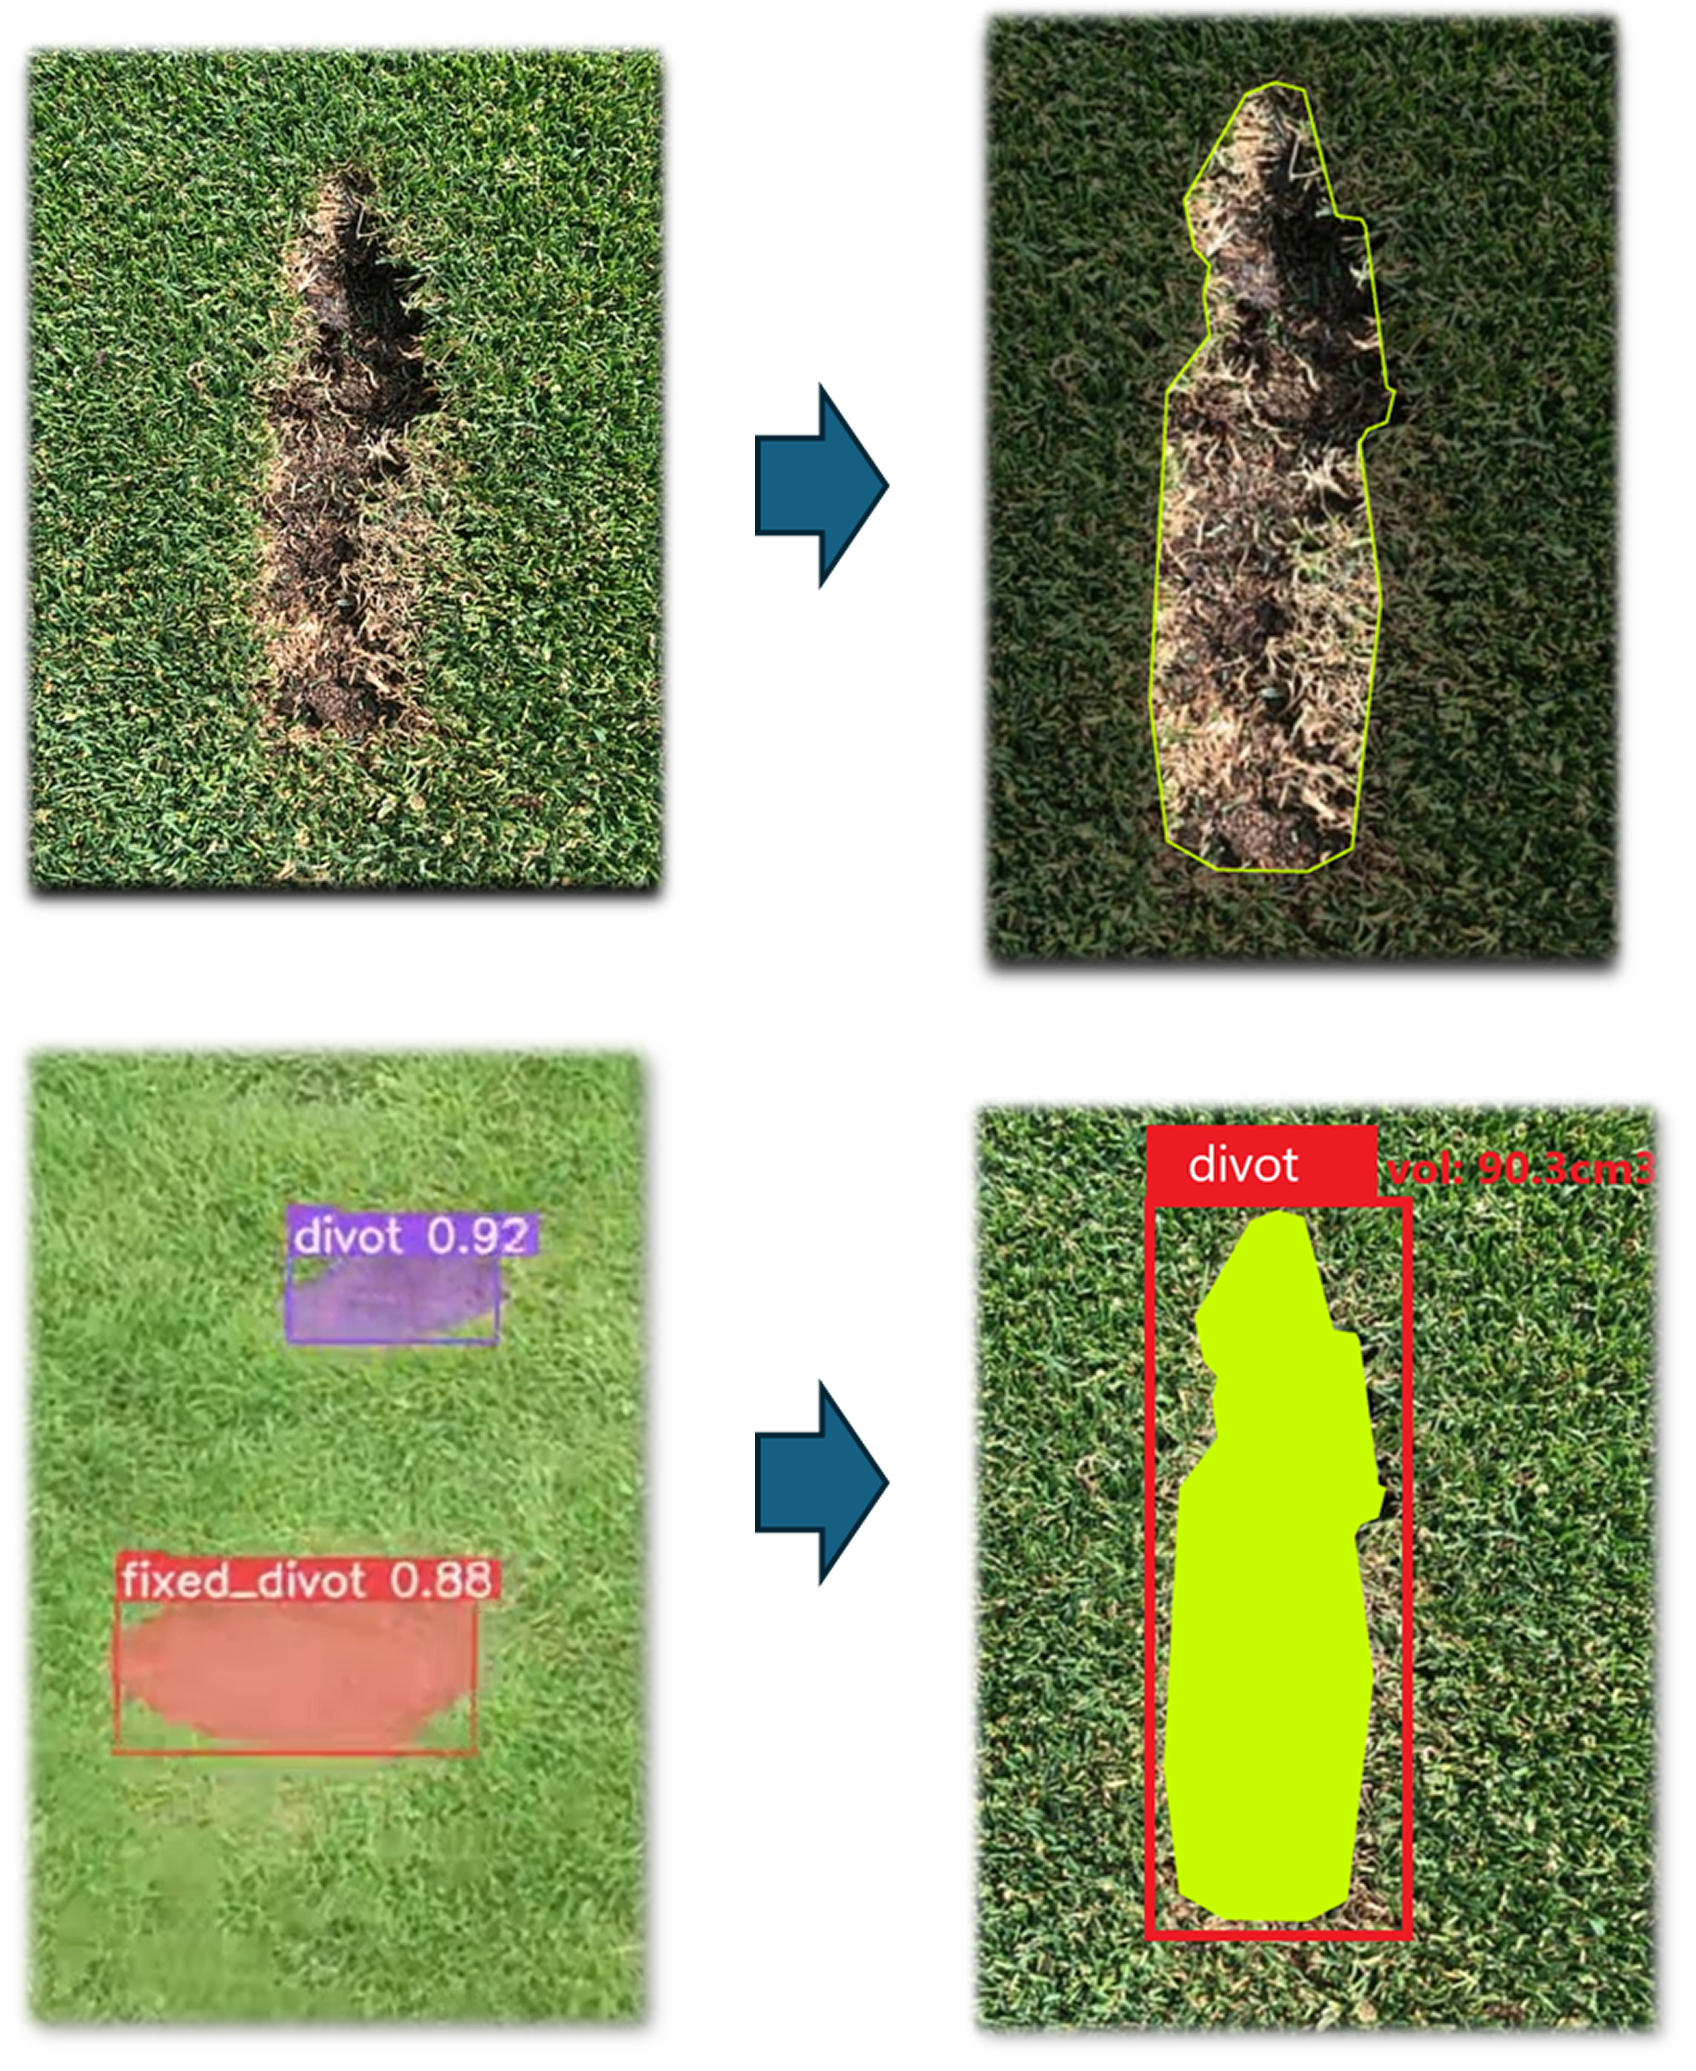
\includegraphics[width=0.9\linewidth]{figures/cv_pipeline_grid.png}
    \caption{The real-time computer vision processing pipeline. The top row shows an original captured image being processed to create a segmentation mask. The bottom row illustrates the subsequent classification and depth analysis steps.}
    \label{fig:cv_processing_pipeline}
\end{figure}

The node subscribes to the \texttt{/camera/color/image\_raw} topic. For each image received, it executes the following sequence:

\begin{enumerate}
    \item \textbf{Instance Segmentation:} The raw image is first passed to the YOLOv11-seg model. The model identifies and generates a precise pixel-level segmentation mask for any object it recognizes as a divot or a fixed divot.

    \item \textbf{Divot Classification:} For each segmented instance, the model provides a classification (either \texttt{divot} or \texttt{fixed\_divot}) along with a confidence score (e.g., \texttt{divot 0.92}). This allows the system to distinguish between areas that need repair and those that have already been serviced.

    \item \textbf{Depth Estimation:} Once a divot is positively identified and segmented, its pixel mask is used to query the corresponding depth data from the RealSense camera's aligned depth stream. While calculating the full volume was deferred as future work, this step confirms that the necessary 3D data can be extracted for a specific, non-rectangular target.
\end{enumerate}

After this pipeline is complete, the results — including the annotated image with segmentation masks, structured details about the detections, and performance metrics — are published to their respective ROS 2 topics for use by the GUI and navigation systems.


\section{Navigation System}
\label{sec:nav_implementation}

\subsection{Purpose}
\label{ssec:nav_intro}
The primary objective of the Navigation System is to provide the GolfBot with precise, real-time positional awareness, enabling it to travel to specific coordinates with centimeter-level accuracy. Standard Global Navigation Satellite System (GNSS) receivers typically offer only meter-level precision, which is insufficient for the targeted task of divot repair. To overcome this limitation, this project implements a Real-Time Kinematic (RTK) positioning system.

The fundamental principle of RTK is to use a stationary base station to calculate and transmit correction data to a moving rover, as illustrated in Figure \ref{fig:rtk_concept}. The base station, whose exact position is known, receives the same satellite signals as the rover. By comparing the signals it receives to its known location, it can determine the atmospheric and timing errors present in the GNSS signal at that moment. These corrections are then sent to the rover, which applies them to its own measurements to achieve a highly accurate position fix.

\begin{figure}[h!]
    \centering
    \includegraphics[width=0.8\linewidth]{figures/rtk.PNG}
    \caption{The operating principle of a Real-Time Kinematic (RTK) system, showing the data flow between the satellite, base station, and rover.}
    \label{fig:rtk_concept}
\end{figure}

\subsection{Hardware Used}
\label{ssec:nav_hardware}
The navigation system is built from two primary hardware components that provide the robot with its sense of position and orientation.

\textbf{ArduSimple simpleRTK2B Starter Kit.}
The core of the high-precision localization system is the ArduSimple simpleRTK2B-LR kit, which provides a complete RTK setup. A visual guide to the components is included in Appendix \ref{chap:appendix_a}, Figure \ref{fig:appendix_ardusimple_kit}. The kit contains:
\begin{itemize}
    \item Two \texttt{simpleRTK2B} boards, each equipped with a multi-band u-blox ZED-F9P GNSS receiver module. One board is configured as the stationary base, and the other as the mobile rover.
    \item A pair of long-range (LR) radio modules and antennas, which establish a direct communication link for transmitting the correction messages from the base to the rover.
    \item Two u-blox multiband GNSS antennas for receiving satellite signals.
\end{itemize}
The base station is designed to be installed at a high point overlooking the operational area. The rover board, mounted on the GolfBot, was configured to output standard \gls{NMEA} messages at a rate of 10 Hz. This provides the robot with RTK-corrected positioning with an expected accuracy of ±2 cm. The rover communicates all its data to the main Jetson controller over a direct USB connection.


\textbf{BNO055 Inertial Measurement Unit (IMU).}
To supplement the GPS data with high-frequency orientation information, a BNO055 IMU was integrated. This sensor provides 9-axis fused data, outputting stable roll, pitch, and yaw angles. The IMU is connected directly to the Arduino Uno via the I2C communication protocol, as shown in Figure \ref{fig:imu_connection}. The specific pin connections are as follows: BNO055 SDA to Arduino A4, SCL to A5, VIN to 5V, and GND to GND.

\begin{figure}[h!]
    \centering
    \includegraphics[width=\linewidth]{figures/arduino-connection.png}
    \caption{Wiring diagram for connecting the BNO055 IMU to the Arduino Uno.}
    \label{fig:imu_connection}
\end{figure}

The orientation data from the IMU is provided as three angles: roll, pitch, and yaw, which describe the robot's rotation around the X, Y, and Z axes, respectively, as illustrated in Figure \ref{fig:imu_axes}.
\begin{itemize}
    \item \textbf{Yaw} (rotation around the Z-axis) represents the robot's heading or turning direction. This is the most critical angle for navigation, as it is used to steer the robot towards a target.
    \item \textbf{Pitch} (rotation around the Y-axis) represents the robot tilting forwards or backwards, such as when traveling up or down a slope.
    \item \textbf{Roll} (rotation around the X-axis) represents the robot tilting side-to-side, which occurs when one wheel is on higher ground than the other.
\end{itemize}
The Arduino is responsible for reading these angles from the sensor and forwarding them to the Jetson controller via a serial-over-USB connection.

\begin{figure}[h!]
    \centering
    \includegraphics[width=0.7\linewidth]{figures/roll.png}
    \caption{Coordinate system and orientation axes (roll, pitch, yaw) of the BNO055 IMU.}
    \label{fig:imu_axes}
\end{figure}

\subsection{Software Implementation}
\label{ssec:nav_software}
The navigation hardware is integrated into the ROS 2 ecosystem through a combination of existing packages and custom-developed Python nodes. These nodes work in parallel to provide the robot with a comprehensive understanding of its global position, local movement, and orientation. While the data from these sensors is not fused through a state estimation filter like a Kalman filter in the current implementation (a topic reserved for future work), they are used cooperatively by higher-level nodes to perform navigation tasks.

\subsubsection{Global Positioning (RTK-GPS)}
The primary source of absolute global position data is the ArduSimple module, which is managed by two key nodes:

\begin{description}
    \item[\texttt{ublox\_gps\_node}] This standard ROS 2 package interfaces directly with the RTK-GPS module via its USB port. It is configured using a YAML file to parse the raw data from the u-blox ZED-F9P receiver. Its sole responsibility is to publish the robot's absolute position (latitude, longitude), altitude, and crucially, the position covariance which indicates the accuracy of the fix. This data is published as a \texttt{sensor\_msgs/NavSatFix} message to the \texttt{/ublox\_gps\_node/fix} topic.

    \item[\texttt{gps\_monitor\_node.py}] This custom utility node subscribes to the \texttt{/fix} topic to provide diagnostics and a human-readable status. It evaluates the horizontal accuracy derived from the covariance matrix to determine the quality of the GPS signal, classifying it as "RTK Fixed," "RTK Float," or standard GPS, and publishes this status for the GUI.
\end{description}

\subsubsection{Orientation and Local Movement}
High-frequency local motion and orientation are provided by the IMU and wheel encoders, managed by their own dedicated nodes.

\begin{description}
    \item[\texttt{stepper\_imu\_node.py}] As described previously, this node establishes a serial connection with the Arduino microcontroller. The Arduino is programmed to continuously read fused orientation data from the BNO055 sensor. The ROS 2 node parses this serial data, converts the Euler angles (roll, pitch, yaw) into a quaternion, and publishes the result as a \texttt{sensor\_msgs/Imu} message to the \texttt{/imu/data} topic. This provides the critical heading (yaw) information used for steering.

    \item[\texttt{odometry\_node.py}] This node provides a high-frequency, relative measurement of the robot's movement. It subscribes to the \texttt{/left\_vesc/sensors/core} and \texttt{/right\_vesc/sensors/core} topics, which contain wheel encoder data from the motor controllers. Using the principles of differential drive kinematics, the node calculates the robot's change in position and heading based on the difference in distance traveled by the left and right wheels. It publishes this local position estimate as a \texttt{nav\_msgs/Odometry} message to the \texttt{/odom} topic and also broadcasts a TF2 transform for visualization in tools like RViz.
\end{description}

\subsubsection{Proof-of-Concept Navigation and Control}
To validate that the sensor data could be used for closed-loop control, a simple autonomous test was implemented.

\begin{description}
    \item[\texttt{rtk\_test\_node.py}] This node demonstrates the cooperative use of all three data sources to perform a controlled "drive forward one meter" task. When triggered, it subscribes to the \texttt{/ublox\_gps\_node/fix} and \texttt{/imu/data} topics. Its control loop uses the Haversine formula ~\cite{Sinnott_Haversine} to calculate the distance traveled from the starting GPS point, while a proportional controller uses the real-time yaw data from the IMU to maintain a straight heading. Once the target distance is reached, the test concludes. This node successfully validates that the robot can use its sensor data to perform a measured, goal-oriented maneuver.
\end{description}

\section{Mechanical Dispenser}
\label{sec:dispenser_implementation}

\subsection{Purpose}
\label{ssec:dispenser_intro}
The mechanical dispenser is the primary actuator for the GolfBot's repair task. Its purpose is to accurately and reliably deposit a controlled amount of sand-seed mixture directly onto a detected divot. The system is designed to be controlled by the main robot software, allowing for both manual and autonomous triggering of the dispensing action. The core of the mechanism is a stepper motor-driven auger, which allows for precise control over the volume and flow rate of the repair material.
\subsection{Hardware Design and 3D-Printed Components}
\label{ssec:dispenser_hardware}
The dispenser hardware consists of a combination of custom 3D-printed parts and standard electronic components, all managed by the Arduino Uno acting as a dedicated low-level controller.

The main physical component is the dispenser unit itself, which was designed in CAD software and 3D-printed. It consists of a main hopper to hold the sand-seed mixture and an internal auger screw. This auger is directly coupled to a \textbf{NEMA 17 stepper motor}. When the motor rotates, the auger pushes a measured amount of the mixture out through a nozzle at the bottom.

The stepper motor is controlled by an \textbf{A4988 stepper motor driver}, which provides the necessary current and micro-stepping capabilities for smooth and precise motor rotation. The A4988 driver acts as the bridge between the high-level logic of the Arduino and the electrical coils of the stepper motor. The complete wiring for this control system is shown in Figure \ref{fig:stepper_wiring}.

\begin{figure}[h!]
    \centering
    \includegraphics[width=\linewidth]{figures/stepper.png}
    \caption{Wiring diagram for the dispenser's control electronics, showing the connections between the Arduino Uno, the A4988 driver, and the NEMA 17 stepper motor.}
    \label{fig:stepper_wiring}
\end{figure}

The key pin connections are as follows:
\begin{itemize}
    \item \textbf{Arduino to A4988 Driver:} The control signals are sent from the Arduino's digital pins to the driver. The \texttt{STEP} pin is connected to Arduino pin 2, the \texttt{DIR} (direction) pin to Arduino pin 3, and the \texttt{ENABLE} pin to Arduino pin 8.
    \item \textbf{Power to A4988 Driver:} The driver's motor logic (VDD) is powered by the Arduino's 5V pin. The high-power motor supply (VMOT) is connected to a dedicated 12V DC-DC converter.
    \item \textbf{A4988 Driver to NEMA 17 Motor:} The four output pins of the driver (2B, 2A, 1A, 1B) are connected to the corresponding wires of the stepper motor's two coils.
\end{itemize}

\subsection{Software Integration in ROS}
\label{ssec:dispenser_software}
The software for the mechanical dispenser is split between a high-level ROS 2 node running on the Jetson and low-level firmware running on the Arduino microcontroller. This common robotics pattern allows the Jetson to handle complex logic while the Arduino manages the precise, real-time control of the stepper motor.

\subsubsection{Arduino Firmware}
The Arduino is flashed with a C++ sketch (\texttt{stepper\_controller\_with\_imu\_simple.ino}) that uses the \texttt{AccelStepper} library to manage the motor. This library is crucial as it handles the generation of the precise electrical pulses required to drive the stepper motor and can manage smooth acceleration and deceleration profiles.

For robustness and simplicity in the final implementation, the key motor performance parameters were hardcoded directly in the Arduino sketch. The maximum speed was set to 2000 steps/second and the acceleration to 2000 steps/second², values that were found to be reliable during testing. The firmware's primary role is to listen for single-character commands over the USB serial port.

\subsubsection{ROS 2 Control Node (\texttt{stepper\_imu\_node.py})}
The \texttt{/stepper\_imu\_node} is the bridge between the ROS 2 ecosystem and the Arduino. In its role as a dispenser controller, it performs two main functions:
\begin{enumerate}
    \item \textbf{Manual Control:} It subscribes to the \texttt{/joy} topic. When the operator presses the designated "start" button (A button) on the gamepad, the node sends an 'R' (Run) character over the serial port to the Arduino. When the "stop" button (B button) is pressed, it sends an 'S' (Stop) character.
    \item \textbf{Autonomous Control:} The node also subscribes to the \texttt{/dispense\_sand} topic. This allows higher-level autonomy nodes (like \texttt{align\_and\_repair\_node}) to programmatically control the dispenser by publishing 'R' or 'S' commands to this topic.
\end{enumerate}

\subsubsection{Configuration and Parameters}

To allow for easy tuning during development, the \texttt{stepper\_imu\_node.py} is designed to be highly configurable through a YAML parameter file (an example is provided in Appendix \ref{chap:appendix_a}, Listing \ref{lst:stepper_yaml}). While the final Arduino firmware uses hardcoded values, the ROS 2 node still declares and loads these parameters, which would be used by a more advanced, configurable version of the Arduino firmware. The key parameters defined in \texttt{stepper\_config.yaml} include:
\begin{description}
    \item[\texttt{port} \& \texttt{baud\_rate}:] Defines the serial port and communication speed for the Arduino.
    \item[\texttt{max\_speed} \& \texttt{acceleration}:] Allows the desired motor speed and acceleration to be set from the launch file.
    \item[\texttt{button\_start} \& \texttt{button\_stop}:] Defines which gamepad buttons are used to manually control the dispenser.
\end{description}
This parameter-driven design in the ROS 2 node makes the system flexible and easy to adapt for future enhancements without needing to modify the core Python code.

\section{Graphical User Interface (GUI)}
\label{sec:gui_implementation}

\subsection{Purpose}
\label{ssec:gui_intro}
To provide a user-friendly way to monitor and control the GolfBot, a custom Graphical User Interface (GUI) was developed. The purpose of the GUI is to serve as a central control panel, consolidating all critical data streams into a single dashboard. This allows an operator to see what the robot sees, monitor its status in real-time, and switch between manual and autonomous modes of operation.

\subsection{Software and Framework}
\label{ssec:gui_software}
The GUI is implemented as a standalone ROS 2 node, \texttt{golfbot\_gui\_node.py}. The user interface itself was built using Python's standard \textbf{Tkinter} library. Tkinter was chosen for its simplicity and the fact that it is included with standard Python installations, making the GUI portable and easy to run.

The \texttt{golfbot\_gui\_node.py} script integrates ROS 2 functionality with the Tkinter GUI by running them in parallel. As shown in the code, the standard ROS 2 \texttt{rclpy.spin()} function, which is responsible for processing incoming messages from subscribers, is executed in a separate background thread. This allows the main thread of the program to be dedicated to running the Tkinter main loop, which handles drawing the window and updating its widgets, ensuring that the user interface remains responsive while continuously receiving data from the robot.

\subsection{Functions, Features, and Control}
\label{ssec:gui_features}
The GUI is organized into a three-panel layout, as shown in Figure \ref{fig:golfbot_gui}, to provide a clear and organized presentation of information.

\begin{figure}[h!]
    \centering
    \includegraphics[width=\linewidth]{figures/GUI.PNG}
    \caption{The GolfBot Control Panel, showing the three-panel layout with real-time data.}
    \label{fig:golfbot_gui}
\end{figure}

\begin{description}
    \item[Left Panel (Control and GPS):] This panel contains the primary operational controls and global positioning status. It features a button to toggle the robot between "Manual Mode" and "Autonomous Mode" by publishing a boolean message to the \texttt{/is\_autonomous\_mode} topic. Below the controls, it displays the current latitude, longitude, and RTK fix status from the GPS.

    \item[Center Panel (Camera View):] The largest panel is dedicated to the live video feed from the \texttt{/camera/divot\_detection/image\_raw} topic. This view shows the operator exactly what the robot sees, including the real-time output of the YOLO model. As seen in the figure, detected divots are overlaid with segmentation masks, bounding boxes, and key calculated metrics such as estimated dimensions, area, volume, and the horizontal (H-Offset) and vertical (V-Offset) distance from the center of the camera frame.

    \item[Right Panel (Robot and System Status):] This panel displays local odometry data (X, Y, and Heading) and detailed information about the primary divot currently being targeted. At the bottom, a "System Status" section provides simple connection indicators (e.g., "Camera: Connected") for key hardware, giving the operator an at-a-glance confirmation that all subsystems are online.
\end{description}

% %Section: Computer Vision System
% Introduction/Purpose: A brief one-paragraph reminder of the goal: to detect divots from a camera feed.
% Data Set Collection and Preprocessing: This is pure implementation.
% How did you collect the 689 images? (e.g., "Images were collected over several days at the Maynooth University campus golf facility under varying lighting conditions...")
% How did you use Roboflow? Describe the process of uploading, annotating the two classes (divot and fixed_divot), and exporting the dataset.
% What specific data augmentations did you apply? Mention the exact transformations like rotation (e.g., +/- 15 degrees), brightness changes (e.g., +/- 25), etc., that expanded the dataset to 1,653 images.
% Model Training:
% Describe the training process on Google Colab. Mention the key parameters: 100 epochs, the specific YOLOv11-seg model used, and the fact that you used TPUs.
% Hardware: You described the camera in the Design chapter. Here, you describe its setup.
% "The Intel RealSense D435i was configured using the pyrealsense2 library to stream RGB video at a resolution of 1280x720 and 30 frames per second."
% Software: List the key libraries you used.
% pyrealsense2 for camera interfacing, OpenCV for image manipulation, and the ultralytics Python package for running the YOLO model inference.
% Implementation in ROS: This is critical.
% Describe your ROS 2 node (divot_detection_intel.py).
% Specify the topics it subscribes to (/camera/color/image_raw) and publishes to (/camera/divot_detection/image_raw, /camera/divot_detection/details).
% Mention the message types (sensor_msgs/Image). You could even include a small, simplified code snippet of your main processing loop.

% Section: Navigation System
% Introduction/Purpose: Reminder of the goal: achieve centimeter-level navigation.
% Hardware Used: Again, focus on the configuration.
% "The ArduSimple simpleRTK2B rover module was configured to output NMEA sentences at 10 Hz over USB."
% "The BNO055 IMU was interfaced with the Arduino, which was programmed to read the fused orientation data and send it over its serial port."
% Software Implementation:
% Explain how you used the ublox_gps_node ROS 2 package to read the data from the ArduSimple module and publish it to the /fix topic.
% Describe your stepper_imu_node.py, explaining how it reads the serial data from the Arduino and publishes it as a sensor_msgs/Imu message on the /imu/data topic.
% This is the perfect place to describe the simple "lawnmower" search algorithm you implemented for autonomous coverage.


% Section: Mechanical Dispenser
% Introduction/Purpose: Reminder of the goal: dispense a controlled amount of sand/seed mix.
% Hardware Design and 3D-Printed Components: You are exactly right with your idea for this section.
% In the Design chapter, you described what it looks like and where it is.
% Here, in Implementation, you describe how it performs. "The auger was designed in Fusion 360 and 3D-printed using PLA. Through a series of tests, it was calibrated to determine its output rate. Running the NEMA 17 stepper motor for X seconds at Y speed dispenses an average of Z grams of the sand-seed mixture. The hopper has a total volume of..."
% Software Integration in ROS:
% Explain the simple serial protocol you created (e.g., sending the character 'R' to run the motor and 'S' to stop it).
% Describe the part of your stepper_imu_node.py that sends these characters to the Arduino's serial port when a joystick button is pressed.
% You could include the simple Arduino code snippet (if (Serial.available() > 0) ...) that listens for these commands and drives the A4988 stepper driver.


% Section: Graphical User Interface (GUI)
% Introduction/Purpose: To provide teleoperation and system monitoring.
% Software and Framework: Describe what you used to build it. (e.g., "The GUI was developed as an RQT plugin using Python and the PyQt5 framework.")
% Functions, Features, and Control:
% Detail what the user can see and do. Show a screenshot.
% "The GUI displays the live camera feed, the annotated divot detection feed, the current RTK GPS status (Fixed, Float, None), and provides buttons for manual control, starting the autonomous mode, and triggering the dispenser."
